\newpage
\begin{sol}
\begin{enumerate}[label=\textbf{(\alph*)}]
\item Our differential equation is:
$$-\frac{\hbar^2}{2m}\frac{d^2}{dx^2}\Psi+(V(x)-E)\Psi$$
Defining $x=au$, then we have $d(au)^2=a^2(du^2)$. Then dividing through $V_0$ we define the characteristic energy as $e\equiv \frac{E}{V_0}$, getting:
$$-\frac{\hbar^2}{2mV_0a^2}\frac{d^2\Psi}{du^2}+(v(x)-e)\Psi$$
where:
$$v(x)=\begin{cases}0 & 0<u<1 \\
1 & 1<u<2\end{cases}$$
Notice that coefficient for the first term is just $\frac{1}{z_0^2}$. Therefore, our final dimensionless differential equation is:
$$-\frac{1}{z_0^2}\Psi''+(v(x)-e)\Psi=0$$
We can solve this via mathematica to obtain $E_1$ and $E_2$.
\begin{center}
    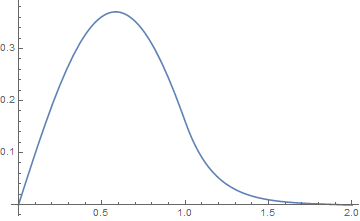
\includegraphics[width=0.35\linewidth]{Images/E1.png}
    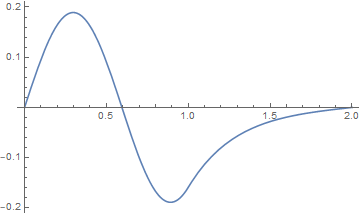
\includegraphics[width=0.35\linewidth]{Images/E2.jpg}
\end{center}
The next two energies (for when $E>V_0$) occurs approximately at $e=1.205$ and $e=1.563$.
\item The eighth excited state has an energy of $e=3.558$, corresponding to the following wavefunction:
\begin{center}
    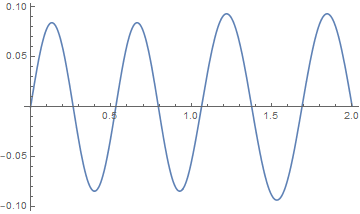
\includegraphics[width=0.4\linewidth]{Images/E8.png}
\end{center}
We have approximately $A_L=0.85$ and $A_R=0.9$ such that $\frac{A_L}{A_R}\approx 0.94$ which is extremely close to the De Broglie approximation, where the ratio would be equal to one.
\end{enumerate}
\end{sol}